\documentclass[conference]{lib/IEEEtran}
\usepackage{graphicx}
\usepackage{babel}
\usepackage[utf8]{inputenc}
\IEEEoverridecommandlockouts
\usepackage{xspace}
% \usepackage{cite}
\usepackage{amsmath,amssymb,amsfonts}
\usepackage{algorithmic}
\usepackage{textcomp}
\usepackage{xcolor}
% \def\BibTeX{{\rm B\kern-.05em{\sc i\kern-.025em b}\kern-.08em
%     T\kern-.1667em\lower.7ex\hbox{E}\kern-.125emX}}
\usepackage{hyperref}
\hypersetup{colorlinks=true, allcolors=black}
\usepackage{subcaption}
\usepackage{mdframed}
\usepackage[colorinlistoftodos,prependcaption,textsize=tiny]{todonotes}
\newcounter{todocounter}
\newcommand{\toreview}{}
\newcommand{\reffig}[1]{Figure \ref{fig:#1}\xspace}

\ifx\toreview\undefined
  \newcommandx{\nota}[2][1=]{}
  \newcommand{\hl}[1]{}

  \newcommandx{\notahl}[2][1=]{}
  \newcommand{\hlhl}[1]{}
  \newcommandx{\notake}[2][1=]{}
  \newcommand{\hlke}[1]{}
  \newcommandx{\notafa}[2][1=]{}
  \newcommand{\hlfa}[1]{}
\else
  % \newcommandx{\nota}[2][1=]{
  %   \stepcounter{todocounter}
  %   \todo[linecolor=red,backgroundcolor=red!25,bordercolor=red,#1]{[\thetodocounter] #2}}
%   \newcommand{\hl}[1]{\colorbox{red!25}{#1}}
  % 
  \newenvironment{highlight}{\begin{mdframed}[backgroundcolor=red!25]}{\end{mdframed}}
  % \newenvironment{myHeartEnv}
  % {\color{purple}{\heartsuit}\kern-2.5pt\color{green}{\heartsuit}}
  % {\text{ forever}}

  % \newcommandx{\notahl}[2][1=]{\stepcounter{todocounter}\todo[
  %   linecolor=green,
  %   backgroundcolor=green!25,
  %   bordercolor=green,#1]{[Helio \thetodocounter] #2}}
  % \newcommand{\hlhl}[1]{\colorbox{green}{#1}}

  % \usepackage{cancel}
  % \newcommandx{\notake}[2][1=]{\stepcounter{todocounter}\todo[
  %   linecolor=yellow,
  %   backgroundcolor=yellow!25,
  %   bordercolor=yellow,#1]{[Kelton \thetodocounter] #2}}
  % \newcommand{\hlke}[1]{\colorbox{yellow}{#1}}

  % \newcommandx{\notafa}[2][1=]{\stepcounter{todocounter}\todo[
  %   linecolor=blue,
  %   backgroundcolor=blue!25,
  %   bordercolor=blue,#1]{[Faria \thetodocounter] #2}}
  % \newcommand{\hlfa}[1]{\colorbox{blue!30}{#1}}

  % \usepackage[showframe,layoutvoffset=0mm,includeall,tmargin=15mm,bmargin=20mm]{geometry}
  % \marginparwidth=34mm
  % \hoffset=-25mm
  % \textwidth=165mm
\fi


\SetAlFnt{\small }
\setlength{\algomargin}{1em}

\makeatletter
\if@twocolumn
\newcommand{\whencolumns}[2]{
#2
}
\else
\newcommand{\whencolumns}[2]{
#1
}
\fi
\makeatother

\begin{document}

\title{IoT Data Stream Novelty Detection:
Design, Implementation and Evaluation [DRAFT]\thanks{CNPq}}

\author{
  \IEEEauthorblockN{Luís Puhl, Guilherme Weigert Cassales, Hermes Senger, Helio Crestana Guardia}\\
  \IEEEauthorblockA{Universidade Federal de São Carlos, Brasil \\
    https://orcid.org/\{0000-0003-4029-2047,
    0000-0003-1273-9809,
    0000-0001-5010-747X\}
  }
  % \IEEEauthorblockN{Hermes Senger}\IEEEauthorblockA{\textit{Universidade Federal de São Carlos}, Brasil \\hermes@ufscar.br}\and
    % \IEEEauthorblockN{Guilherme Weigert Cassales}\IEEEauthorblockA{\textit{Universidade Federal de São Carlos}, Brasil \\gwcassales@gmail.com}
    % \and
    % \IEEEauthorblockN{4\textsuperscript{th} Given Name Surname}
    % \IEEEauthorblockA{\textit{dept. name of organization (of Aff.)} \\
    % \textit{name of organization (of Aff.)}\\
    % City, Country \\
    % email address or ORCID}
}

\maketitle

\newcommand{\refminas}{\textit{Ref}\xspace}
\newcommand{\mfog}{\textit{MFOG}\xspace}
\newcommand{\iot}{IoT\xspace}
\newcommand{\arch}{IDSA-IoT\xspace}
\newcommand{\nids}{NIDS\xspace}
\newcommand{\nd}{DSND\xspace}
\newcommand{\minas}{MINAS\xspace}

\begin{abstract}
% cenário, problema, 
  The ongoing implementation of the Internet of Things (\iot) is sharply
  increasing the number and variety of small devices on edge networks and,
%   break to 2-3 lines
  following this increase, the attack opportunities for hostile agents also
  increases, requiring more from network administrators and the need for tools
  to detect and react to those threats.
  % 
  One such tool are the Network Intrusion Detection Systems (\nids)
  which captures and analyses network traffic,
  acting when a known attack or a new pattern is detected.
  For a network security tool to operate in the context of edge and
  \iot it has to comply with processing, storage and energy
  requirements alongside traditional requirements for stream and network
  analysis like accuracy and scalability.
  % 
  Using a previously defined architecture (\arch),
  we address the construction and evaluation of a distributed \nids
  with the Data Stream Novelty Detection (\nd) algorithm MINAS
  employing C and MPI library.
%   apresentar a estratégia,
  % 
  We discuss the algorithm steps, how it can be deployed in a distributed
  environment, the impacts on the accuracy and evaluate performance and
  scalability using a cluster of constrained devices commonly found in \iot
  scenarios.
  % 
  % We found an increase of \textit{A 0.0} processed network flow descriptors per
  % core added to the cluster.
  % Also \textit{B 0.0\%} and \textit{C 0.0\%} change in
  % \textit{F1Score} in the tested datasets when stream was unlimited in speed and
  % limited to \textit{0.0 z MB/s} respectively.
  We found a marginal ($2$ to $4\%$) difference in true positive (hits) between
  original, serial and distributed executions, consuming a months worth of flow
  descriptors in $300$ seconds.
%   concluindo que é viável e barato utiliar este tipo de abordagem
  \todo[inline]{Manter IDS? Fazer novelty detection distribuído utilizando recursos na borda, em pequenos dispositivos buscado escalabilidade (?) e baixa latência, 
  Os resultados mostram que ..., permitindo concluir que ... }
\end{abstract}

\ifdefined\IEEEkeywords
\begin{IEEEkeywords}
  % Detecção de Novidades, Detecção de Intrusão, Fluxos de Dados, Computação Distribuı́da, Computação em Névoa, Internet das Coisas.
  novelty detection, intrusion detection, data streams,
  distributed system, edge computing, internet of things
\end{IEEEkeywords}
\else
\keywords{
novelty detection \and intrusion detection \and data streams \and
distributed system \and edge computing \and internet of things
}
\fi


% \listoftodos
% \todototoc

\section{Introduction}


% \todo{poderia trocar esses surveys por mais novos ou menos preditivos e mais acertvivos}

% A survey released by Gartner estimated about 20 billion devices connected to the
% Internet by 2020, many of them through the IoT \cite{gartner_forecast_2017}.
% More recently, Statista predicted that the total number of such devices will
% reach 38 billion by 2025, and 50 billion by 2030 \cite{statista-iot}.
The Internet of Things (\iot) brings together a wide variety of devices,
including mobile, wearable, consumer electronics, automotive and sensors of
various types.
% 
Such devices can either be accessed by users through the Internet or connect
to other devices, servers and applications,
with little human intervention or supervision
\cite{Tahsien2020,abane2019,haddadpajouh2019survey,Shanbhag2015}.
% 
Security and privacy is a major concern in the \iot, especially regarding
% devices like smart home assistants and wearable
devices having access to user personal data like
location, health and many other sensitive data \cite{sengupta2020comprehensive}.
% 
Furthermore, if compromised, such devices can also be used to attack other
devices and systems, steal information, cause immediate physical damage or
perform various other malicious acts \cite{Kolias2017mirai}.
% 
As an additional concern, \iot devices likely have a long lifespan, less frequent
software patches, growing diversity of technologies combined with lack of
control over the software and hardware of such devices by the host organization
(where they are deployed), which considerably increases the attack surface.

% A study reveals that nearly $20\%$ of organizations have experienced at least one
% IoT-based attack in the last three years.
% The study shows that most organizations have no control over the origin and
% nature of software and hardware used by the connected devices.
% To protect against these threats, the IoT industry's spending on security is
% estimated to be around USD $\$\,3.1$ billion in 2021 \cite{gartner_it_glossary_2018}, 
% which includes the development of tools
% and services to improve asset discovery and management, software security
% evaluation, hardware % testing 
% and penetration testing.

% i.e. 'id est', which means "that is."
% e.g. 'exempli gratia', which means "for example."
% {\color{red} muito próximo de \cite{Cassales2019a}}
Because most \iot devices have limited resources (i.e., battery, processing,
memory and bandwidth), configurable and expensive algorithm-based
security techniques are not usual, giving way to network based approaches 
% may not fit 
\cite{Zhou2017}.
Machine Learning (ML) techniques, for instance, have been studied for years to detect attacks
from known patterns or to discover new attacks at an early stage
\cite{buczak2016survey,mitchell2014survey}.
A recent survey \cite{Tahsien2020} shows that ML based methods are a
promising alternative which can provide potential security tools for the \iot
network making them more reliable and accessible than before.

Despite the promising use of ML to secure \iot systems, studies found in the
literature \cite{buczak2016survey,mitchell2014survey,Tahsien2020} are limited to
traditional ML methods that use static models of traffic behavior.
% With traditional ML methods, the data set is static and can be traversed
% repeatedly, and the detection of new attack patterns requires a new cycle of
% training, testing, and dissemination of new models.
Most existing ML solutions for network-based intrusion detection cannot maintain
their reliability over time when facing evolving attacks \cite{Viegas2019,AndreoniLopez2019}.
Unlike traditional methods, stream mining algorithms can be applied to intrusion
detection with several advantages, such as:
\begin{enumerate*}[label=(\emph{\roman*})]
    \item processing traffic data with a single read;
    \item working with limited memory (allowing the implementation in small
    devices commonly employed in edge services);
    \item producing real-time response; and
    \item detecting novelty and changes in concepts already learned.
\end{enumerate*}

% Nao tinha mencionado quais previous works...
% {\color{red} %This paper elaborates on the previous work in the following aspects.

% {\color{red} Adicionar referencias e relacionados. Argumentar que além de \nids,
% \nd para \iot tem outras aplicações}

% CATRACA \cite{AndreoniLopez2018,AndreoniLopez2019} SBRC AndreoniLopez2019
% BigFlow \cite{Viegas2019}
Given the recent \cite{Viegas2019,AndreoniLopez2019,DaCosta2019a} use of Data Stream Novelty
Detection (\nd) in network data streams, this paper shows the effects of
adapting these mechanisms to edge services for use in \iot environments.
Our proposal, called \mfog, adapted the \arch
architecture \cite{Cassales2019a} using the \nd algorithm \minas
\cite{Faria2013Minas,Faria2016minas}, making it suitable to run
% (as it was already tested in a similar \iot scenario) 
on a distributed system composed of small devices with limited
resources on the edge of the network.
% Our implementation can be fully executed on the edge, thus avoiding any dependency
% and high latency of cloud resources.
% We proposed and implemented dMINAS, a distributed extension
% of MINAS \cite{Faria2016minas} (a novelty detection for data streams).
Using our newer version of the \minas algorithm, we have experimentally evaluated 
% through experimental methodology, 
how the distribution 
% the chosen novelty detection algorithm \minas
affects the capability to detect changes (novelty) in
traffic patterns and its impact on the computational efficiency.
Finally, some distribution strategies and policies for the data stream
novelty detection system are discussed.
% }

% \begin{figure}[hb]
%     \centering
%     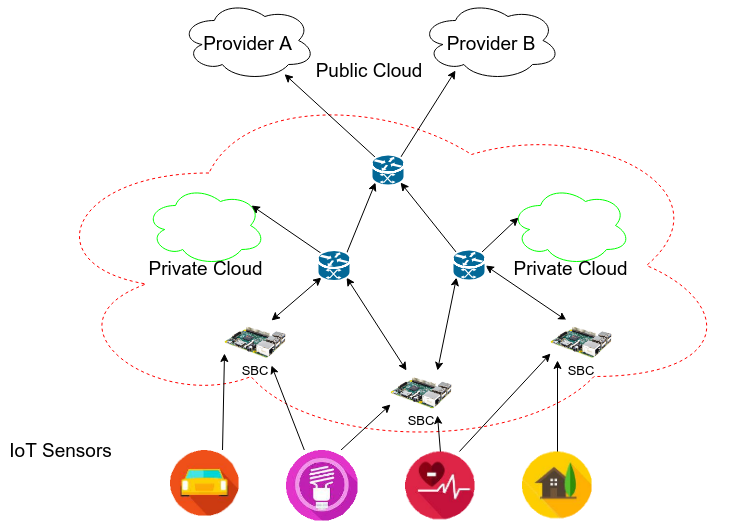
\includegraphics[width=0.5\linewidth]{figures/cassalesimgs-000.png}
%     \caption{\arch \cite{Cassales2019a} physical architecture and deployment scenario overview.}
%     \label{fig:mfog-phy-arch-cloud}
% \end{figure}

This paper is organized as follows:
% Section \ref{sec:related} presents the related works.
Section \ref{sec:minas} reviews the chosen \nd algorithm \minas.
A distributed extension of \minas, including its
implementation and evaluation are presented in Section \ref{sec:prop}
and in Section \ref{sec:experiments} we show how we evaluated \mfog and
the discuss results we found.
Finally, Section \ref{sec:conclusion} summarizes the main findings and presents
possible future work.

% \todo{Parei aqui a redação da Introdução.Deixei grifado em vermelho o
% paragrafo que fala das contribuições. Talvez com um pequeno esforço em
% especificar uma versão distribuida do MINAS teriamos uma extensão do mesmo. }

% Desafios de arquitetura e validação:

% - Construção de um protótipo da arquitetura IDSA-IoT:
%   - Kafka (Python): Distribuição e balanceamento pelo cluster kafka, hipótese refutada.
%   - Flink (Java ou Scala): Execução do cluster nos dispositivos de névoa, hipótese refutada.
%   - MPI (C e Python): Execução do cluster nos dispositivos de névoa, hipótese aceita.
% - Reimplementação do algoritmo MINAS com fidelidade:
%   - Duas versões: a descrita e a implementação de referência (em Java).
%   - Resolução: utilizar a descrição, não *seguir* a imp. referência, apenas como ponto de comparação. Exemplos:
%     - Definição de raio `r = f * σ` (fator vezes desvio padrão) para `r = max(distance)` (distância máxima);
%     - Tamanho do buffer de desconhecidos e frequência de execução do passo de detecção de novidade;

% \begin{highlight}
% Expected results:
% A system that embraces and explores the inherent distribution of fog computing
% in a IoT scenario opposing regular systems where data streams are collected and
% centralized before processing;
% Impact assessment of the impact of distributed, regional flow characteristics,
% local vs global vs distributed forgetting mechanism and other policies.

% IDS characteristics and description of physical scenario.

% MINAS characteristics.

% Distribution and IDSA-IoT architecture.
% \end{highlight}

% This paper is structured as follows:
% Section \ref{sec:related} presents previous works that addresses related
% problems and how they influenced our solution.
% Section \ref{sec:implementation} address our proposal, the work done, issues
% found during implementation and discusses parameters and configurations options
% and how we arrived at our choices.
% Section \ref{sec:experiments} shows experiments layouts and results, we
% compare serial and distributed implementation's metrics for validation,
% we also evaluate communication delay effects on classification metrics and
% conclude with the speedup per core and overall maximum stream speed.
% Section \ref{sec:conclusion} summarizes the research results and presents our
% final conclusions and future works.


% ----------------------------------------------------------------------------------------------------------------------
\section{Related Work}
\label{sec:related}

Network Intrusion Detection based on Machine Learning is not a novel concept.
The plethora of network applications and 
ways of exploiting them, motivate using automated means to detect known and novel attacks. 
% the interest of teach a machine how to detect a novel attack is formed.
There are, though, open questions and challenges on this subject, such as
reducing false positive rate and detecting attacks in a timely fashion \cite{DaCosta2019a}.

A few recent works inspired our work, such as: BigFlow \cite{Viegas2019}
employing Apache Kafka and Apache Flink for distributed stream processing,
four algorithms (Hoeffding Tree, OzaBoosting, Leveraging Bag) and one Ensemble
from the Massive Online Analysis (MOA) library \cite{MOA}, and
evaluating with package stream dataset solving the time constraint for \nids;
CATRACA \cite{Lopez2018,AndreoniLopez2019a}, in a similar way, uses 
Apache Kafka and Apache Spark for stream processing and also achieves
a timely and scalable \nids.

% % {\color{red} muito próximo de \cite{Cassales2019a}}
% 6LoWPAN is a standard defined by the IETF in RFC 6282, to transmit data with
% IpV6 and other protocols on low power wireless devices using IEEE 802.15.4 in
% the lower layers. However, this technology still lacks protection and security
% mechanisms. %\cite{dos-6lowpan-iot, Hybrid-ids-arch-iot, SVELTE}.
% %
% For instance, in \cite{dos-6lowpan-iot}, signature detection is used to detect
% DoS and UDP flood attacks. The architecture uses a probe to promiscuously listen
% the whole traffic of a 6LoWPAN network and sends the data to analysis on a
% non-constrained host.
% %Results were expressed by flood metrics, as the number of packets in the network.
% The work in \cite{SVELTE} proposed an hybrid IDS which focuses on specific
% routing attacks, such as sink-hole and selective-forwarding. Higher complexity
% tasks which demand more computational resources are executed on the border
% router, while simpler tasks execute on constrained nodes. Results were expressed
% by metrics as recall and memory and energy consumption.
% % 
% The work in \cite{Hybrid-ids-arch-iot} proposed the use of anomaly detection to
% identify internal routing attacks, and signature detection to identify external
% attacks. Anomaly detection was tested with simulated attacks, while signature
% detection used a subset of NSL-KDD. They used the recall and FAR as metrics.

A three-layer architecture (composed of WSN, Fog and Cloud) with focus on fault
tolerance in disaster scenarios is proposed in \cite{Fault-tolerance-disaster}.
Fog computing is used to execute ML functions and data aggregation. Experiments
used real data collected from sensors. The metrics used included precision,
recall and accuracy.
%
The work in \cite{Kalis} proposed an hybrid IDS which collects information about
the environment and activates specific modules to mitigate each kind of attack.
Experiments were made in a real environment and metrics used were recall,
precision and resource consumption (CPU and RAM).
%
Smart cities scenarios also employ IoT to measuring and monitoring tasks.
%\cite{IoT-arch-smartmeter,scalable-anomaly-detection-smart-city,DS-based-IDS-SmartGrid}.
In \cite{IoT-arch-smartmeter}, the authors propose an architecture that uses
three stream mining methods based on ML to characterize water and energy
consumption behavior, predict consumption, and detect incidents.
The metrics used to express results include water and energy consumption.
%
The work in \cite{scalable-anomaly-detection-smart-city} also aimed to identify
anomalies in a water distribution network and proposes a three layer
architecture (sensors, base stations and datacenter).
The second layer performs time-sensitive tasks, thus reducing latency, while
third layer provides storage and aggregates the results of the second layer with
historical data to generate more accurate information.
Water distribution measures were used, comparing the values of the predictions
with the actual measurements.
%
Intrusion detection for smart cities, based on data mining techniques running on
an unrestricted devices is proposed in \cite{DS-based-IDS-SmartGrid}.
Experiments using KDD99 data are presented and the metrics used were precision,
Kappa, memory consumption, time, FAR, and FNR.


Table \ref{tab:summary} summarizes the discussion on the related work.
Note that some works use data from KDD99 or derived from this dataset.
Collected two decades ago, KDD is no longer representative of current attack
patterns and IoT environments.
Some works used traces captured from local infrastructure, which provide
realistic evaluation, but lack of reproducibility.
Some works used data produced by intentional simulated attacks, designed by the
same people who designed the detection techniques.
This can bring unrealistic advantages to the detection methods.
Also, it is worth noting that most articles used metrics like FAR, recall, and
accuracy.
Although widely adopted in classical scenarios, such metrics are inaccurate for
stream processing \cite{GAMA2010}.

\begin{table*}[htb]
\caption{Summary of related works}
\centering
\begin{scriptsize}
% \begin{tabularx}{\textwidth}{ l m{2cm} | m{2cm} l m{2cm} | m{2cm} | m{2cm} | m{2cm} }
\begin{tabularx}{\textwidth}{l|l|X|X|X}
% \begin{tabularx}{\textwidth}{l|l|X|X|m{3.0cm}}
% Trabalho & Platforma  & Técnica & DataSet & Métricas \\
Work                                         & Platforms    & Technique & DataSet & Metrics\\\hline\hline
% Kasinathan et al
\cite{dos-6lowpan-iot}                       & 6LoWPAN      & Suricata & Real data with metasploit & Accuracy, packets/second\\\hline
% Sheikhan and Bostani
\cite{Hybrid-ids-arch-iot}                   & 6LoWPAN      & Hybrid - MR OPF & NSL-KDD and simulated attacks & FAR and recall\\\hline
% Raza et al
\cite{SVELTE}                                & 6LoWPAN      & DAG analysis & No information & Recall, energy and memory consumption\\\hline
% Furquim et al
\cite{Fault-tolerance-disaster}              & WSN          & MLP of Weka & Real data & MAE, RMSE, R², R, accuracy, recall, precision, specificity\\\hline
% Midi et al
\cite{Kalis}                                 & WSN          & Independent modules, each with one technique & Trace replay and attack injection & Recall, accuracy, memory and CPU consumption\\\hline
% Lloret et al
\cite{IoT-arch-smartmeter}                   & Smart City   & Clustering, MLP and statistical models & Real data from meters & Water and energy consumption\\\hline
% Diffalah et al
\cite{scalable-anomaly-detection-smart-city} & Smart City   & LiSA, smoothing function & Real data & Outliers, comparison between simulation and collected data\\\hline
% Faisal et al
\cite{DS-based-IDS-SmartGrid}                & Smart Grid   & 7 MOA classifiers & KDD99 & Accuracy, Kappa, memory consumption, time, FAR and FNR \\\hline
\end{tabularx}
\label{tab:summary}
\end{scriptsize}
\end{table*}

% ----------------------------------------------------------------------------------------------------------------------
% - Escrever! Corpo:
%   - Proposal (retomar problema {iot, sec, ND}, objetivo, soluções {minas, paralelismo, distribuído, ~~py-kafka, flink,~~ mpi}, propor uma solução)
%   - Implementation (mpi, c, data-structures, data-flow, )
%   - Experiments (rpi, cluster, `evaluate.py`)
%   - Results
%   - Conclusion
% - Demonstrar o paralelismo com figura de pipeline (time vs instruction)


\section{Proposal}
\label{sec:prop}
% Proposal:
%  - retomar problema {iot, sec, ND};
%  - objetivo;
%  - soluções {minas, paralelismo, distribuído, ~~py-kafka, flink,~~ mpi}
%  - propor uma solução

Amid of \iot expansion in multiple fields, from industry to daily life,
the constant threat of intrusion, subversion (overthrow), denial of service
or any other unexpected detrimental behavior by any component of a system or
external actors is a prospect looming over many systems administrators.
Following that reasoning, new \nids and other autonomous and analytics system
surveillance tools are being proposed, many employing technics such as Anomaly
and Novelty Detection.

These tools require the network packet traffic to be constantly analysed,
aggregated into flow descriptors and further processed in a classification
and any Intrusion Detection.
This requirement in turn, requesting more computing power at the edge.
While requesting more computing power in a cloud environment is trivial and
inexpensive, the same cannot be said 

\begin{highlight}
Fog computing infrastructure aims to offload
computing resources from cloud providers by placing edge
devices closer to end-users and/or data sources.

Objective: Distributed novelty detection in streams using limited hardware.

Previous attempts to attain the objective of distributed fast
\end{highlight}

The overall organization of components, connections and interactions with external
actors is shown in \ref{fig:mfog-phy-arch-cloud},
from bottom left to top right: sensor network; fog containing gateway router
and novelty detection cluster; cloud storage for model, alarms and statistics
and; human supervisor addressing alarms and statistics.

\begin{figure*}[h]
  \centerline{
    \begin{subfigure}{.5\textwidth}
      \centering
      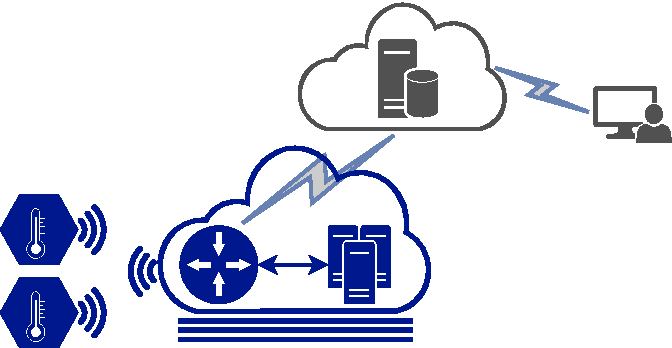
\includegraphics[width=0.9\linewidth,page=1]{figures/mfog-arch-fisica.svg.pdf}
      \caption{\mfog physical architecture overview with cloud model storage.}
      \label{fig:mfog-phy-arch-cloud}
    \end{subfigure}
    \begin{subfigure}{.5\textwidth}
      \centerline{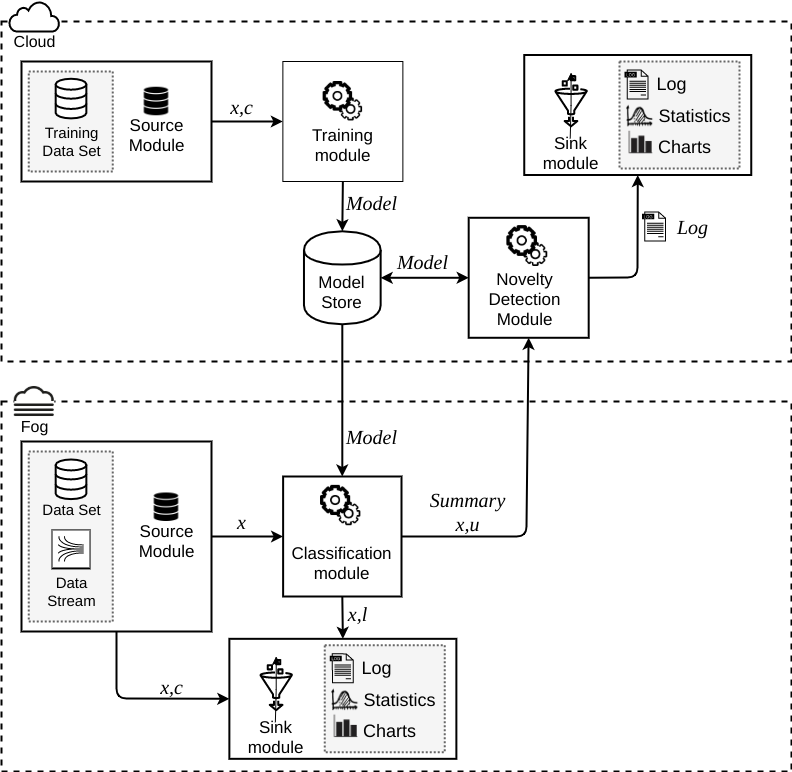
\includegraphics[width=0.9\linewidth]{figures/mfog-arch-v2_en.png}}
      \caption{\mfog components and communications overview.}
      \label{fig:mfog-architecture}
    \end{subfigure}
  }
  \caption{Architecture overview.}
  \label{fig:arch-overview}
\end{figure*}

\subsection{Implementation}\label{sec:implementation}

The original MINAS algorithm has a companion implementation (\refminas)
written in Java using MOA library base algorithms such as K-means and CluStream.
% \refminas employs Java's double, a $64 bits$ number whose precision is not
% absolutely necessary and, as it is often necessary to shuffle between nodes via
% network and a small economy could be made with only a float number with $32 bits$.
Another difference between \refminas and \mfog is cluster radius calculation
from the distances of elements forming the cluster and the cluster's center,
where the former uses the maximum distance, the latter uses the standard deviation
of all distances as described in \cite{Faria2016minas}.

% Desafios de implementação:
% <!--
% - Definição de raio: desvio padrão das distâncias versus distancia máxima;
% - Atualização do micro-cluster limita-se à atualização do atributo \texttt{T};
% - Remoção de exemplos na implementação de referência é feita somente para o algoritmo \textit{CluStream};
% - Inclusão de borda: algoritmo inclui ($<=$), referência não inclui ($<$);
% - Seguiu-se as mesmas divergências anteriores para comparação dos resultados com a implementação referência;
% - Inclusão da borda;
% - Comportamento do mecânismo de \textit{sleep-model} não está definido, portanto não está ativo;
% - Processo de clusterização é limitado ao algoritmo \textit{K-Means}. Algoritmo \textit{CluStream} não está implementado;
% - -->
% - `Double vs Float`:
%   - Na implementação de referência, java double é utilizado;
%   - Na nova implementação duas versões foram testadas e a diferença de precisão entre as duas é de `5 E-8`;
%   - **Solução:** Use `float32` e economize os bits já que haverá comunicação entre nós e módulos;
% - Formato do fluxo de saída:
%   - Implementação de referência utiliza a tripla `(id, classe, etiqueta)`;
%   - Primeira implementação em C utiliza `(id, clusterLabel, clusterId, clusterRadius, label, distance, secondDistance)`;
%   - Segunda implementação utiliza dupla `(id, label)`;
%   - Na etapa de avaliação, independente de versão, o fluxo original é lido;
%   - **Solução:** O formato mínimo é `(id, label)`;

The stream format for input and output also of note.
Input information needed is the value of the item, this value is a number
sequence of length $d$ (referenced as dimension).
In addition to the value for evaluation and training purposes the class
identifier as single character, optimality an unique item identifier
(\textit{uid}) can be provided.
For output information and format the decision isn't so clear as we can't
predict future system integrations needs like only novelty alarms or every
item's original value with assigned label so, we have a compromise and put only
enough information for the Evaluation Module (where the full information
from the testing file or stream can de accessed) meaning the format can be
defined as a tuple containing \textit{uid} and assigned label.

% - Reprocessamento dos exemplos utilizados para atualização do modelo:
%   - Muda o comportamento do operador de fluxo de `Map` para `Flatmap`, ou seja,
%     requer outro fluxo de saída para a transmissão de padrões novidade (alarmes);
%   - Para reclassificação a definição de raio é modificada de `r = f * σ` (fator
%     multiplicando desvio padrão) para `r = max(distance)` (distância máxima);
%   - Passível da crítica de *overfitting*. Isto é, este processo pode
%     inflar a métrica de precisão;
%   - **Solução:** *em aberto*;

Another implementation decision related to the output stream is whether or not
to reprocess, and add to the output stream, examples in the unknown buffer after
the novelty detection procedure, meaning one item can be classified once as
unknown and again with a label.
Our tests using this technique had increased true positives when compared to
not using it.
However this changes the stream operator behavior from a \textit{Map} to a
\textit{FlatMap} having duplicate entries on the output stream as previously
mentioned.
Regardless of choice the classification of the unknown buffer after a model
update, using the full model or just the added set of clusters, is done to
remove the examples ``consumed'' in the creation of a new cluster in the internals
of the clustering algorithm.
% This removal can be made less complex if using only new clusters 

% Próximos desafios:
% - Distribuição e paralelização para minimização de latência entre novo item no fluxo e sua classificação:
%   - Tempo de passagem da instância pelo classificador;
%   - Volume máximo do sistema;
%   - Diferenças de precisão de acordo com a carga;

For \mfog the Message Passing Interface (MPI) library was used.
In MPI programming, multiple processes of the same program are created by the
runtime and each process instance receives a rank parameter, for \mfog this
parameters indicate if the process is root, rank $0$, or leaf otherwise.
Beyond this division, each process also operates two threads, for the root
there is a sampler and detector threads, for the leafs each has a model receiver
thread and multiple classifier threads.
The overall sequence of creation is shown in \ref{fig:mfog-mpi-life}.

\begin{figure}[htb]
  \centerline{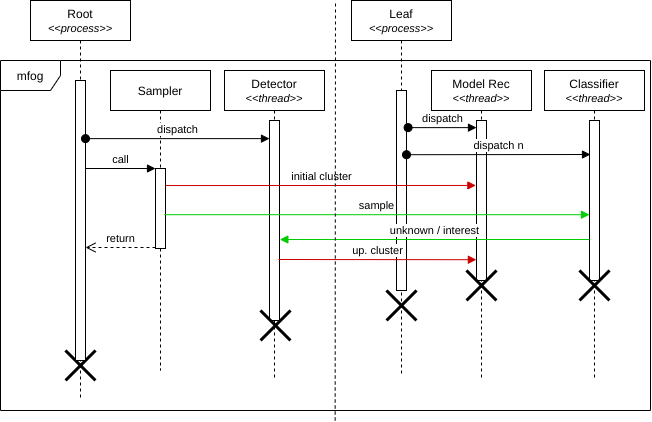
\includegraphics[width=0.5\textwidth]{figures/mfog-arch-mpi.png}}
  \caption{\mfog life line overview.}
  \label{fig:mfog-mpi-life}
\end{figure}

\begin{highlight}
Polices

- Detecção de novidades e manutenção de modelo em ambiente distribuído:

  - Mecanismo de ND local (síncrono) vs nuvem quanto à atraso de definição de modelo
    (nesse ponto é onde a hipótese prevê maior diferença, grande ponto de interesse);

  - Mecanismo de esquecimento local vs global (modelo único ou por nó);

  - Atraso na reclassificação dos desconhecidos;
\end{highlight}

The Evaluation Module was also build following reference techniques like
multi-class confusion matrix with label-class association
\cite{Faria2016minas}
to extract classification quality metrics.


% ------------------------------------------------------------------------------
\section{Experiments and Results}
\label{sec:experiments}

For the experimental setup we dedicated 3 Raspberry Pi single board computers
connected via Gigabit Ethernet Switch forming a simple cluster.
This cluster stored all source code, binaries (compiled and linked in place) and
datasets, being accessed via our laboratory network over Secure Shell (SSH).
All experiments were executed in this cluster for isolation of otherwise unforeseen
variations.

The dataset used is the December 2015 segment of
Kyoto 2006+ Dataset\footnote{Available at \url{http://www.takakura.com/Kyoto\_data/}}
(Traffic Data from Kyoto University's Honeypots)
\cite{Song2011}.
This segment was filtered (from $7\:865\:245$ instances) to only examples
associated to known attack types identified by existing IDS, and attack types
with more than $10\:000$ instances for significance as done by \cite{Cassales2019a}.
% , this removes 46,390 instances. TODO: revisar, pois 7M != 700K.
The remaining instantes then were transformed by normalization, transforming
each feature value space (e.g. IP Address, Duration, Service) to the
Real interval $[0, 1]$.
The result is stored in two sets, training set and test set, using the holdout
technique filtering in only normal class resulting in $72\:000$ instances for
training set and $653\:457$ for test set, containing $206\:278$ $N$ (normal) class
and $447\:179$ $A$ (attack) class.

% Count per class
%            id
% class        
% A      447179
% N      206278

% \begin{quote}
%   For the experiments, we used the Kyoto 2006+ dataset
%   which contains data collected from 2006 to December 2015.
%   We selected examples from one month, December, 2015. Only the examples of known
%   attack types and known IDS alert code with a minimum of 10,000 occurrences (for
%   significance) were considered. The offline training was performed with 72,000
%   examples (i.e., 10\% of the dataset) using the holdout technique.
%   \cite{Cassales2019a}
% \end{quote}

\begin{highlight}
O que quer testar com os experimentos.
\begin{itemize}
  \item Tese: Mostrar que detecção por novidade e classificação continua viável em fog.
  \item Seria inviável por conta do atraso de distribuição de modelo e,
  \item limitação pelo hardware pequeno.
  \item MFOG: Um Agregador Regional, instalado na FOG, que observa a rede local.
\end{itemize}

Como realizou (cenário, rpi, setup, coleta de métricas).

Quais resultados obteve.

Como interpretar os resultados.
\end{highlight}

% \hl{BEGIN Oritações de leitura das métricas e visualizações.}

\subsection{Metrics and Visualizations}

There are two broad evaluation metrics for each experiment:
a time mesure extracted by using \emph{GNU Time 1.9} and,
a set of qualitative mesures extracted by a python program.
The first metric is straightforward and is the time measure of the full program execution.
The latter metric is not as simple and for its extraction required a
purposely build python program.
This program takes two inputs, the test dataset and the captured output stream,
and outputs the confusion matrix, label-class association,
final quality summary with: Hits (accuracy), Misses (Err), Unknowns (UnkR); and
stream visualization chart with per example instance summary with novelty label markers.

For clarity, it is necessary to detail how to interpret and compare each metric,
as for some it is trivial but others are not so straightforward.

In the confusion matrix $M = m_{ij} \in \mathbb{N} ^{c \times{} l}$,
computed by our evaluation program,
each row denotes one of the datasets original (actual) class
and each column denotes the marked (predicted) label present in the captured output stream.
Thus, each cell $M_{c, l}$ contains the count of examples from the test dataset of class $c$
found in the output stream with the label $l$ assigned by the under evaluation experiment.
For the dataset under use, original classes are \emph{``N''} and \emph{``A''}, and
for the labels we have the training class \emph{``N''}, unknown label \emph{``-''} and
the novelties $i \in \mathbb{N}$.

Added to the original confusion matrix $C$ are the rows \emph{Assigned} and
\emph{Hits}.
The former represents which original class $c$ (or if unknown, \emph{-}) the
label $l$ is assigned to, this is computed by using the original class if
$c = l$ or by associated novelty label to original class as described in
\cite{DeFaria2015} section 4.1.
The latter row, \emph{Hits}, shows the true positive count for each label,
computed by coping the value of the cell $M_{c, l}$ where the label is the same
and the class $c$ is the value in the above \emph{Assigned} row.
The \emph{Hits} row is also used to compute the overall accuracy.

For the metric summary table, six metrics from two sources are displayed.
Three metrics \emph{Hits} \emph{Unknowns} \emph{Misses} represented as ratio of the
captured output stream, extracted from the evaluation python
program, computed as follows:
\emph{Hits} (overall accuracy) is the summation of the homograph row in the
extended confusion matrix;
\emph{Unknowns} is the count of examples in the captured output stream marked
with the unknown label \emph{-};
\emph{Misses} is the count of all examples in the captured output stream marked
with a label distinct from the \emph{Assigned} original class and are not marked
as unknown.
\emph{Time}, \emph{System} and \emph{Elapsed} represented in seconds,
are extracted from \emph{GNU Time}.
\emph{Time} is the amount of CPU seconds expended in user-mode
(indicates time used doing CPU intensive computing, e.g. math);
\emph{System} is the amount of CPU seconds expended in kernel-mode
(for our case it indicates time doing input or output);
\emph{Elapsed} is the real-world (wall clock) elapsed time
(indicates how long another system or person had to wait for the result).
To compare the time metric is simple, the lower time taken, the better.

Lastly, the stream visualization chart shows the summary quality metrics
(\emph{Hits} \emph{Unknowns} \emph{Misses})
computed for each example in the captured output stream.
This summary is computed for each example but it uses the \emph{Assigned} row
computed previously to evaluate \emph{Hits}, other metrics are derived as
described before.
Therefore, horizontal axis (x, domain) plots the index of the example and the
vertical axis (y, image) shows the metric computed until that example index on the captured
output stream.
Adding to the summary metrics, novelty label markers are represented as vertical
lines indicating \emph{when} in the captured output stream a new label first
appeared.
Some of the novelty label markers include the label itself ($l \in \mathbb{N}$)
for reference as if showing every label would turn this feature unreadable due
to overlapping.

% \hl{END Oritações de leitura das métricas e visualizações.}

\subsection{Results Discussion}

Four main experiments need detailed discussion:
(a) reference implementation of Minas (\refminas) \cite{Faria2016minas};
(b) new implementation in serial mode;
(c) new implementation in single-node, multi-task mode and
(d) new implementation in multi-node, multi-task mode.
Each experiment uses the adequate binary executable, initial model
(or training set for the reference implementation) and test set
to compute a resulting output stream which is stored for qualitative evaluation.
The summary of all four experiments is shown in Table \ref{tab:exper-summary}.

\begin{table}[h]\begin{center}
  \caption{Experiments Collected Metrics Summary}
  % \begin{tabular}{l|r|r|r|r}
%          &    Exp. (a)  & Exp. (b)   & Exp. (c)    & Exp. (d)   \\\hline
% Hits     &     0.305618 &   0.298438 &    0.312416 &    0.312478    \\\hline
% Misses   &     0.676049 &   0.657843 &    0.664061 &    0.663802    \\\hline
% Unknowns &     0.018333 &   0.043717 &    0.023521 &    0.023718    \\\hline
% Time     &  2761.830000 &  80.790000 &  522.100000 &  207.140000    \\\hline
% System   &     7.150000 &  11.510000 &   47.770000 &  157.610000    \\\hline
% Elapsed  &  2772.070000 &  93.030000 &  145.040000 &   95.380000    
% \end{tabular}

% java -ea -classpath bin/minas/revised.jar: NoveltyDetection.MinasRevised datasets/training.csv datasets/test.csv out/revised-java.log true
% 	2761.82 user	7.15 system	46:12.07 elapsed

% ./bin/offline
% 	193.94 user	0.05 system	3:14.04 elapsed

% "./bin/ond
% 	80.79 user	11.51 system	1:33.02 elapsed

% mpirun -n 12 -hostfile ./conf/hostsfile ./bin/tmpi
% 	207.13 user	157.61 system	1:35.38 elapsed

\newcommand{\mr}[1]{\multirow{2}{*}{#1}}

\begin{tabular}{l|r|r|r|r|r}
                & \refminas (a)  & Offline       & Serial (b)      & Single Node (c) & Multi Node (d)  \\\hline
\mr{Hits}       & $\ 199708\ $   &               & $\ 195017\ $    & $\ 204151\ $    & $\ 204191\ $    \\
                & $\ 0.305618\ $ &               & $\ 0.298438\ $  & $\ 0.312416\ $  & $\ 0.312478\ $  \\
\hline
\mr{Misses}     & $\ 441769\ $   &               & $\ 429873\ $    & $\ 433936\ $    & $\ 433767\ $    \\
                & $\ 0.676049\ $ &               & $\ 0.657843\ $  & $\ 0.664061\ $  & $\ 0.663802\ $  \\
\hline
\mr{Unknowns}   & $\ 11980\ $    &               & $\ 28567\ $     & $\ 15370\ $     & $\ 15499\ $     \\
                & $\ 0.018333\ $ &               & $\ 0.043717\ $  & $\ 0.023521\ $  & $\ 0.023718\ $  \\
\hline
Time            & $\ 2761.83\ $  & $\ 194.12\ $  & $\ 80.79000\ $  & $\ 522.1000\ $  & $\ 207.1400\ $  \\\hline
System          & $\ 7.15\ $     & $\  0.075\ $  & $\ 11.51000\ $  & $\  47.7700\ $  & $\ 157.6100\ $  \\\hline
Elapsed         & $\ 2772.07\ $  & $\ 194.27\ $  & $\ 93.03000\ $  & $\ 145.0400\ $  & $\  95.3800\ $  
\end{tabular}


  \label{tab:exper-summary}
\end{center}\end{table}

The first two experiments (a and b) comparison does serve as validation for our
implementation, while the latter three (b, c and d) serves as showcase for
the effects of distribution.

\begin{figure*}[h]
  \centerline{
    \begin{subfigure}{.5\textwidth}
      \centering
      \includegraphics[width=\linewidth]{experiments/revised-java.log.png}
      \caption{Reference Implementation}
      \label{fig:validation-sub-java}
    \end{subfigure}
    \begin{subfigure}{.5\textwidth}
      \centering
      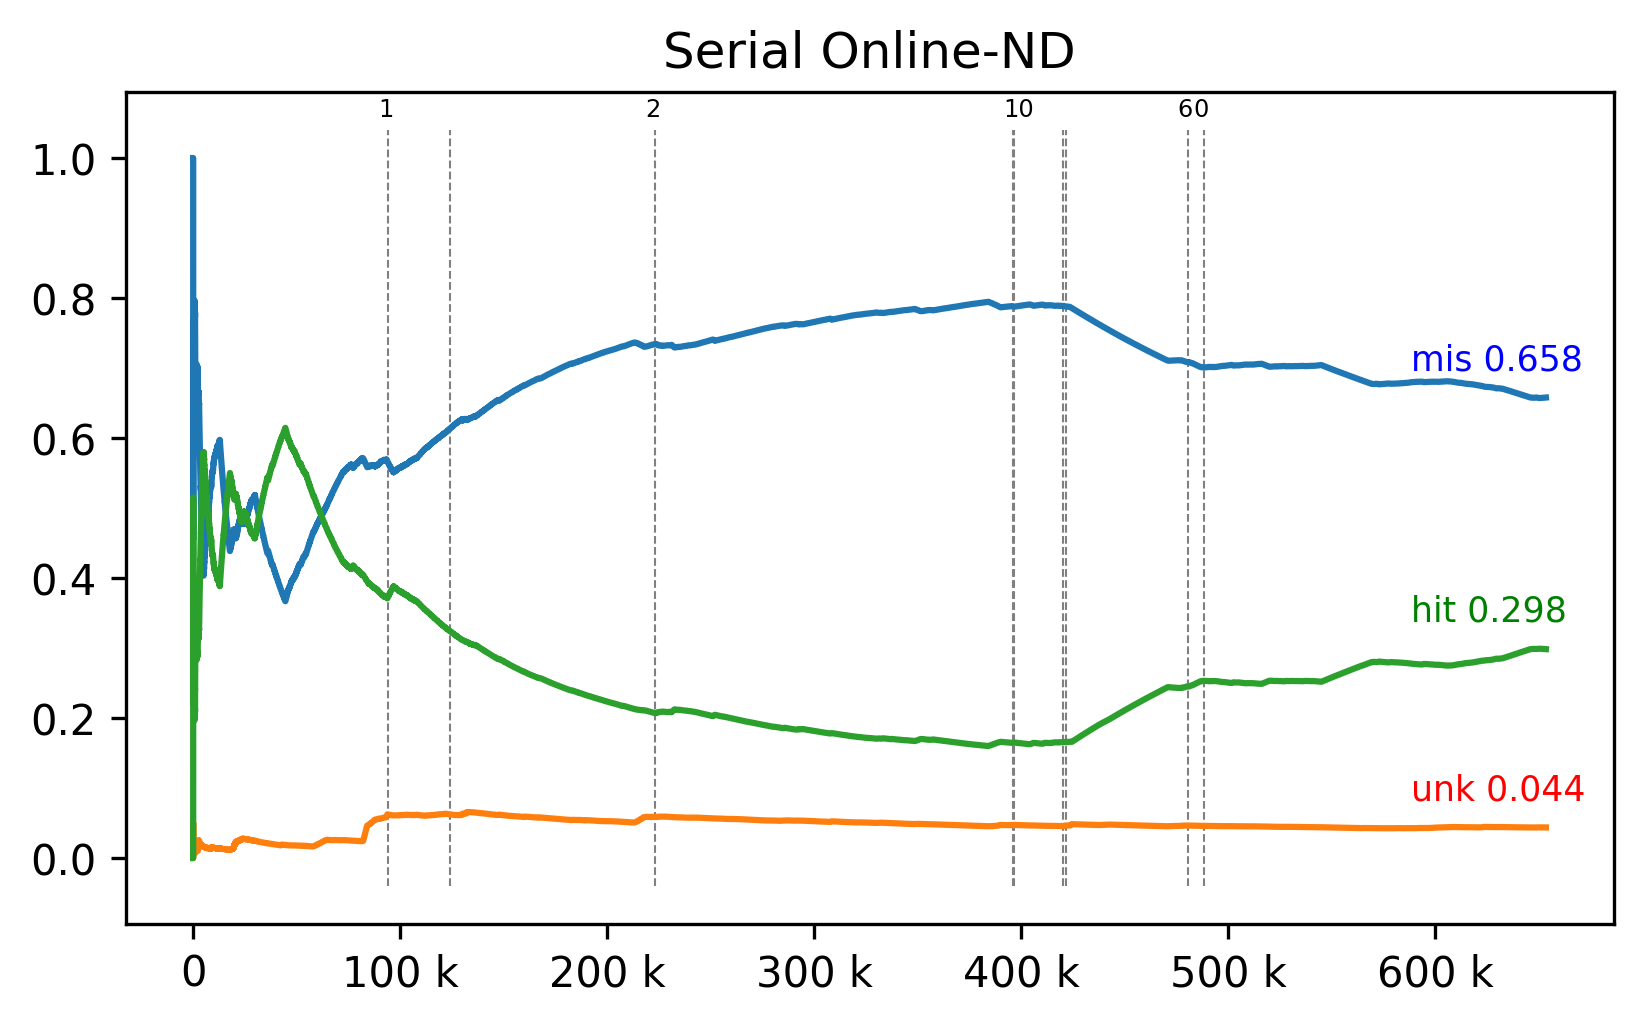
\includegraphics[width=\linewidth]{experiments/online-nd.log.png}
      \caption{Serial Implementation}
      \label{fig:validation-sub-serial}
    \end{subfigure}
  }
  \caption{Validation Comparison: Stream hits and novelties visualization}
  \label{fig:validation-java-serial}
\end{figure*}

\begin{table*}[htb]\begin{center}
  \caption{Reference implementation: Confusion Matrix and Qualitative Metrics}
  \begin{tabular}{l|r|r|r|r|r|r|r|r|r|r|r|r|r|r}

Labels &     - &       N &    1 &    2 &    3 &  4 &   5 &    6 &    7 &     8 &    9 &    10 &   11 &  12 \\\hline
Classes  &       &         &      &      &      &    &     &      &      &       &      &       &      &     \\\hline
\hline
A        &  3774 &  438750 &  123 &  145 &  368 &  8 &  52 &  165 &    1 &  1046 &  161 &  2489 &   71 &  26 \\\hline
N        &  8206 &  193030 &    0 &   79 &   44 &  0 &   0 &    0 &  229 &   181 &  154 &  4066 &  289 &   0 \\\hline
\hline
Assigned &     - &       N &    A &    A &    A &  A &   A &    A &    N &     A &    A &     N &    N &   A \\\hline
Hits     &     0 &  193030 &  123 &  145 &  368 &  8 &  52 &  165 &  229 &  1046 &  161 &  4066 &  289 &  26 
\end{tabular}
% \begin{tabular}{l|r}

% Metric   &        Value \\\hline
% Metric   &              \\\hline
% \hline
% Hits     &     0.305618 \\\hline
% Misses   &     0.676049 \\\hline
% Unknowns &     0.018333 \\\hline
% Time     &  2761.830000 \\\hline
% System   &     7.150000 \\\hline
% Elapsed  &  2772.070000 
% \end{tabular}

  \label{tab:java-matrix}
\end{center}\end{table*}
\begin{table*}[htb]\begin{center}
  \caption{Serial implementation: Confusion Matrix and Qualitative Metrics}
  \begin{tabular}{l|r|r|r|r|r|r|r|r|r|r|r}

Labels &      - &       N &   0 &    1 &    2 &   4 &   5 &  6 &   7 &   8 &  10 \\\hline
Classes  &        &         &     &      &      &     &     &    &     &     &     \\\hline
\hline
A        &  16086 &  429765 &  94 &  995 &  104 &   0 &  23 &  3 &  29 &  46 &  34 \\\hline
N        &  12481 &  193642 &   3 &   94 &    0 &  47 &   0 &  0 &   0 &  11 &   0 \\\hline
\hline
Assigned &      - &       N &   A &    A &    A &   N &   A &  A &   A &   A &   A \\\hline
Hits     &      0 &  193642 &  94 &  995 &  104 &  47 &  23 &  3 &  29 &  46 &  34 
\end{tabular}
% \begin{tabular}{l|r}

% Metric   &      Value \\\hline
% Metric   &            \\\hline
% \hline
% Hits     &   0.298438 \\\hline
% Misses   &   0.657843 \\\hline
% Unknowns &   0.043717 \\\hline
% Time     &  80.790000 \\\hline
% System   &  11.510000 \\\hline
% Elapsed  &  93.030000 
% \end{tabular}

  \label{tab:libc-matrix}
\end{center}\end{table*}

\begin{figure*}[tb]
  \centerline{
    \begin{subfigure}{.5\textwidth}
      \centering
      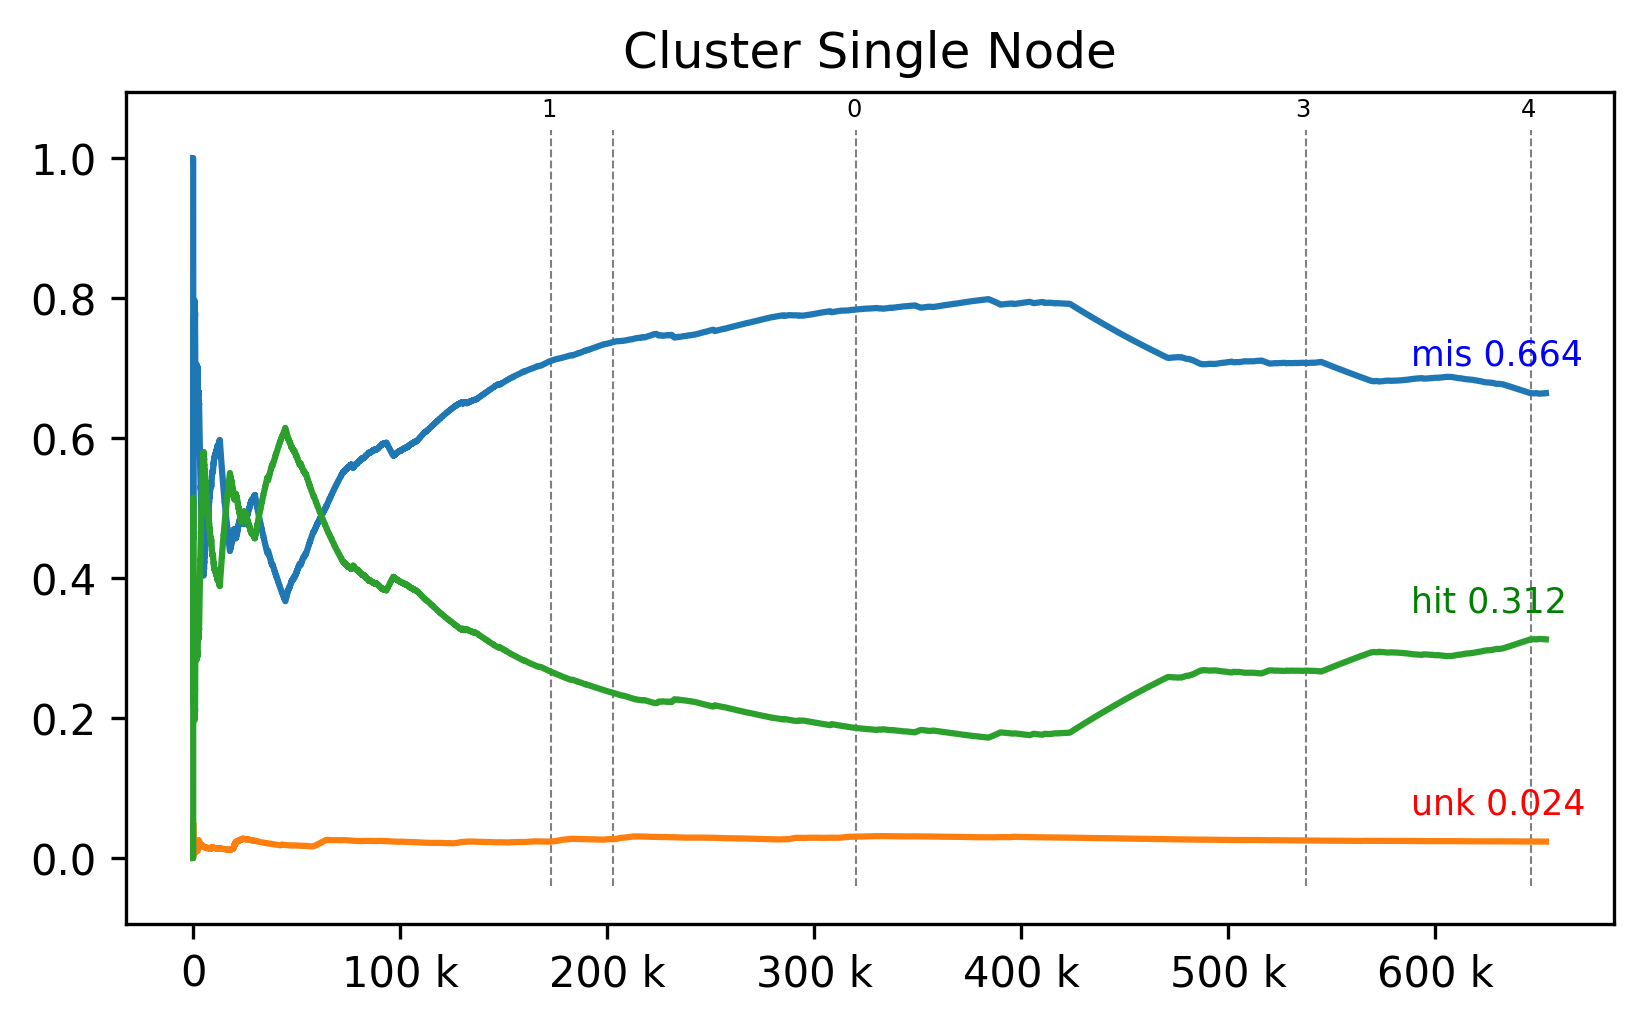
\includegraphics[width=\linewidth]{experiments/tmi-base.log.png}
      \caption{Parallel single-node}
      \label{fig:cluster-sub-single}
    \end{subfigure}
    \begin{subfigure}{.5\textwidth}
      \centering
      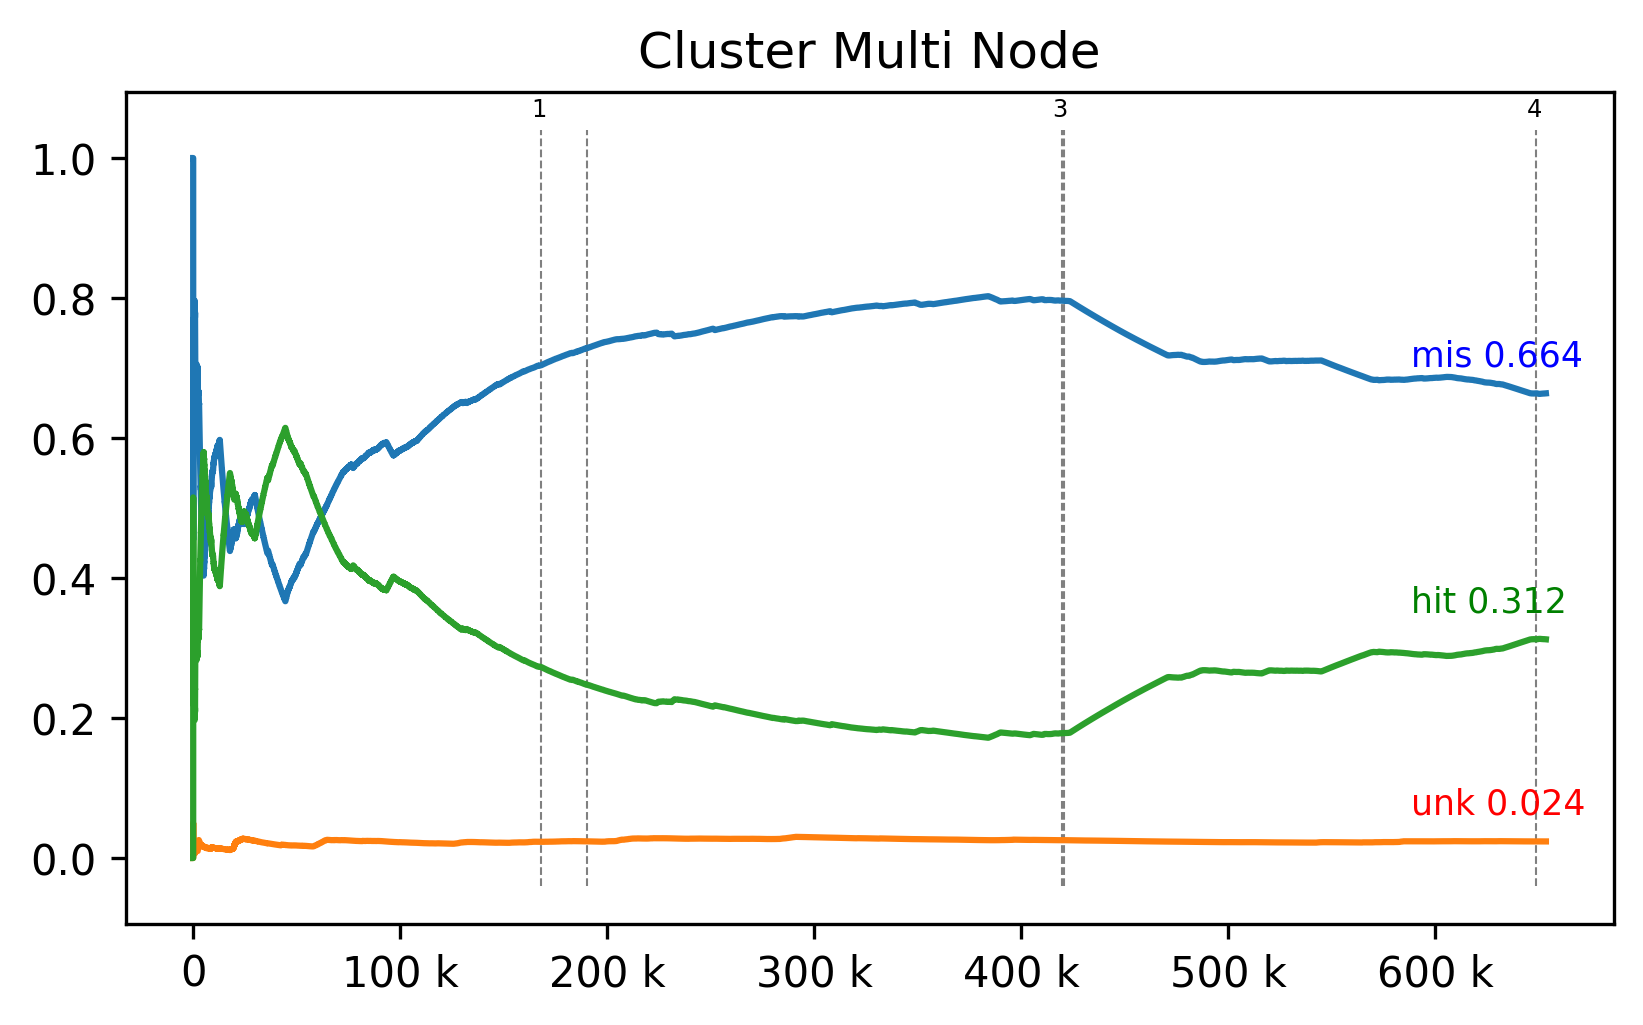
\includegraphics[width=\linewidth]{experiments/tmi-n12.log.png}
      \caption{Parallel multi-node}
      \label{fig:cluster-sub-multi}
    \end{subfigure}
  }
  \caption{Parallelism Comparison: Stream hits and novelties visualization}
  \label{fig:cluster}
\end{figure*}

\begin{table}[htb]\begin{center}
  \caption{Reference implementation: Confusion Matrix and Qualitative Metrics}
  \begin{tabular}{l|r|r|r|r|r|r|r}

Labels &      - &       N &    0 &    1 &   2 &  3 &  4 \\\hline
Classes  &        &         &      &      &     &    &    \\\hline
\hline
A        &  12282 &  433797 &  147 &  952 &   0 &  0 &  1 \\\hline
N        &   3088 &  203019 &   40 &   99 &  27 &  5 &  0 \\\hline
\hline
Assigned &      - &       N &    A &    A &   N &  N &  A \\\hline
Hits     &      0 &  203019 &  147 &  952 &  27 &  5 &  1 
\end{tabular}
% \begin{tabular}{l|r}

% Metric   &       Value \\\hline
% \hline
% Hits     &    0.312416 \\\hline
% Misses   &    0.664061 \\\hline
% Unknowns &    0.023521 \\\hline
% Time     &  522.100000 \\\hline
% System   &   47.770000 \\\hline
% Elapsed  &  145.040000 
% \end{tabular}

  \label{tab:java-matrix}
\end{center}\end{table}
\begin{table}[htb]\begin{center}
  \caption{Serial implementation: Confusion Matrix and Qualitative Metrics}
  \begin{tabular}{l|r|r|r|r|r|r|r}

Labels &      - &       N &    0 &    1 &   2 &  3 &  4 \\\hline
Classes  &        &         &      &      &     &    &    \\\hline
\hline
A        &  12282 &  433797 &  147 &  952 &   0 &  0 &  1 \\\hline
N        &   3088 &  203019 &   40 &   99 &  27 &  5 &  0 \\\hline
\hline
Assigned &      - &       N &    A &    A &   N &  N &  A \\\hline
Hits     &      0 &  203019 &  147 &  952 &  27 &  5 &  1 
\end{tabular}
% \begin{tabular}{l|r}

% Metric   &       Value \\\hline
% \hline
% Hits     &    0.312416 \\\hline
% Misses   &    0.664061 \\\hline
% Unknowns &    0.023521 \\\hline
% Time     &  522.100000 \\\hline
% System   &   47.770000 \\\hline
% Elapsed  &  145.040000 
% \end{tabular}

  \label{tab:libc-matrix}
\end{center}\end{table}

% \setcounter{MaxMatrixCols}{20}
% \begin{table*}[htb]
  %   \begin{center}
    %     \caption{Reference implementation: Confusion Matrix and Qualitative Metrics}
    %     \begin{math}\begin{pmatrix}
      %       - & N & 1 & 2 & 3 & 4 & 5 & 6 & 7 & 8 & 9 & 10 & 11 & 12
%     \end{pmatrix}\end{math}
%     \begin{math}\begin{pmatrix}
%     3774 &  438750 &  123 &  145 &  368 &  8 &  52 &  165 &    1 &  1046 &  161 &  2489 &   71 &  26 \\
%     8206 &  193030 &    0 &   79 &   44 &  0 &   0 &    0 &  229 &   181 &  154 &  4066 &  289 &   0
%     \end{pmatrix}\end{math}
%     \begin{math}\begin{pmatrix}
%       - &       N &    A &    A &    A &  A &   A &    A &    N &     A &    A &     N &    N &   A \\
%       0 &  193030 &  123 &  145 &  368 &  8 &  52 &  165 &  229 &  1046 &  161 &  4066 &  289 &  26 
%     \end{pmatrix}\end{math}
%     \label{math-tab}
%   \end{center}
% \end{table*}

% \begin{figure*}
%   \centering
%   \centerline{
%     \includegraphics[width=0.45\textwidth]{../experiments/revised-java.log.png}
%     \includegraphics[width=0.45\textwidth]{../experiments/revised-java.log.png}
%   }
%   \\
%   \centerline{
%     \includegraphics[width=0.45\textwidth]{../experiments/revised-java.log.png}
%     \includegraphics[width=0.45\textwidth]{../experiments/revised-java.log.png}
%   }
% \label{fig1} 
% \end{figure*}

% \begin{highlight}

% \end{highlight}


% ----------------------------------------------------------------------------------------------------------------------
\section{Conclusion {\color{red} Nao mexer por enquanto}} 
\label{sec:conclusion}

% ----------------------------------------------------------------------------------------------------------------------
\section*{Acknowledgment}

% The preferred spelling of the word ``acknowledgment'' in America is without an ``e'' after the ``g''.
% Avoid the stilted expression ``one of us (R. B. G.) thanks $\ldots$''.
% Instead, try ``R. B. G. thanks$\ldots$''.
% Put sponsor  acknowledgments in the unnumbered footnote on the first page.
The authors thank CNPq (Contract 167345/2018-4).
Hermes Senger also thanks CNPq (Contract 305032/2015-1) and FAPESP (Contract
2018/00452-2, and Contract 2015/24461-2) for their support.


\bibliographystyle{lib/IEEEtran.bst}
\bibliography{refs.bib}
\end{document}
